\section{Приложение <<Тест>>}

\textbf{Задание:} Создать приложение для проведения тестирования. Оно должно содержать:

\begin{enumerate}
    \item Набор вопросов по какой-то теме (и вопросы и ответы должны быть реальные) "--- не менее 10
    \item Вопросы должны выбираться случайным образом.
    \item Вопросы должны быть нескольких типов "--- <<Да/нет>>, Выбор одного ответа, Выбор нескольких ответов, Короткий ответ.
    \item Необходимо создать сообщения для правильного и неправильного ответа (Молодец, Не правильно и т.д.)
    \item Необходимо подсчитать количество правильных ответов и вывести результат.
\end{enumerate}
Вид окна представлен на изображениях \ref{fig:task9_form1},\ref{fig:task9_form2}.
\begin{figure}[H]
    \centering
    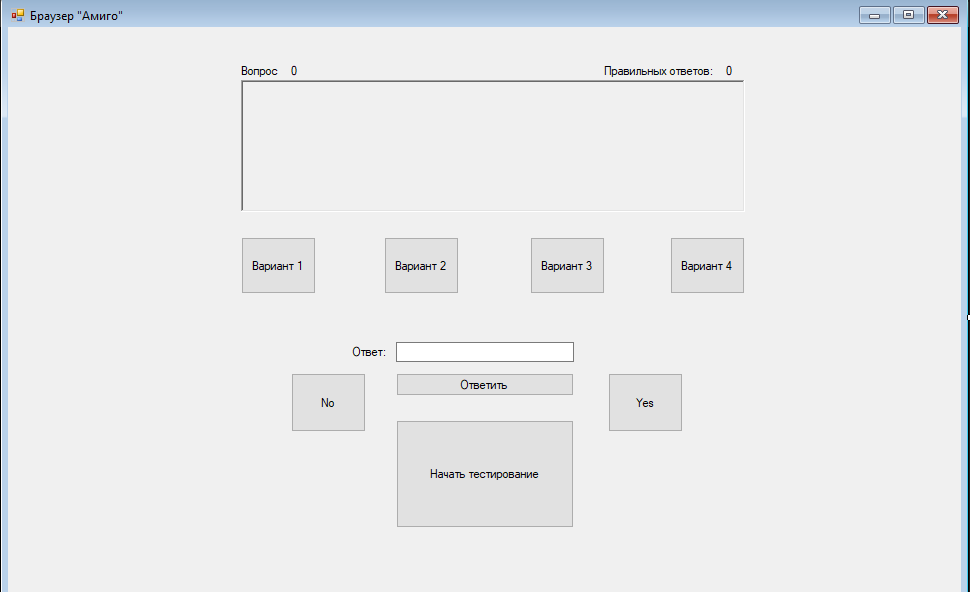
\includegraphics[scale=0.6]{task9/form1.png}
    \caption{Внешний вид формы 1}
    \label{fig:task9_form1}
\end{figure}
\begin{figure}[H]
    \centering
    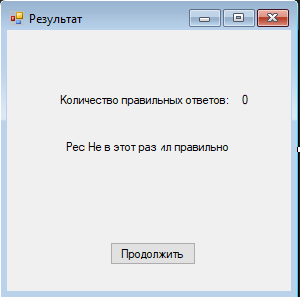
\includegraphics[scale=0.8]{task9/form2.png}
    \caption{Внешний вид формы 2}
    \label{fig:task9_form2}
\end{figure}
У элементов изменены значения некоторых атрибутов. 
Значения измененных атрибутов представлены в таблице \ref{table:params9}.
\begin{longtable}{|l|l|}
    Наименование атрибута & Значение\cr\hline
    \multicolumn{2}{|l|}{Для формы}\cr\hline
    \verb"Text" & \verb"Браузер "Амиго""\cr\hline
    \verb"FormBorderStyle" & \verb"FixedSingle"\cr\hline
    \verb"MaximizeBox" & \verb"False"\cr\hline
    \multicolumn{2}{|l|}{Для кнопки варианта 1}\cr\hline
    \verb"(Name)" & \verb"Option1Btn"\cr\hline
    \verb"Text" & \verb"Вариант 1"\cr\hline
    \multicolumn{2}{|l|}{Для кнопки варианта 2}\cr\hline
    \verb"(Name)" & \verb"Option2Btn"\cr\hline
    \verb"Text" & \verb"Вариант 2"\cr\hline
    \multicolumn{2}{|l|}{Для кнопки варианта 3}\cr\hline
    \verb"(Name)" & \verb"Option3Btn"\cr\hline
    \verb"Text" & \verb"Вариант 3"\cr\hline
    \multicolumn{2}{|l|}{Для кнопки варианта 4}\cr\hline
    \verb"(Name)" & \verb"Option4Btn"\cr\hline
    \verb"Text" & \verb"Вариант 4"\cr\hline
    \multicolumn{2}{|l|}{Для кнопки "Да"}\cr\hline
    \verb"(Name)" & \verb"YesBtn"\cr\hline
    \verb"Text" & \verb"Да"\cr\hline
    \multicolumn{2}{|l|}{Для кнопки "Нет"}\cr\hline
    \verb"(Name)" & \verb"NoBtn"\cr\hline
    \verb"Text" & \verb"Нет"\cr\hline
    \caption{Значения атрибутов элементов в приложении <<Приложение <<Тест>> >>}
    \label{table:params9}
\end{longtable}
После запуска приложения появляется окно (см. рисунок \ref{fig:exec9})
\begin{figure}[H]
    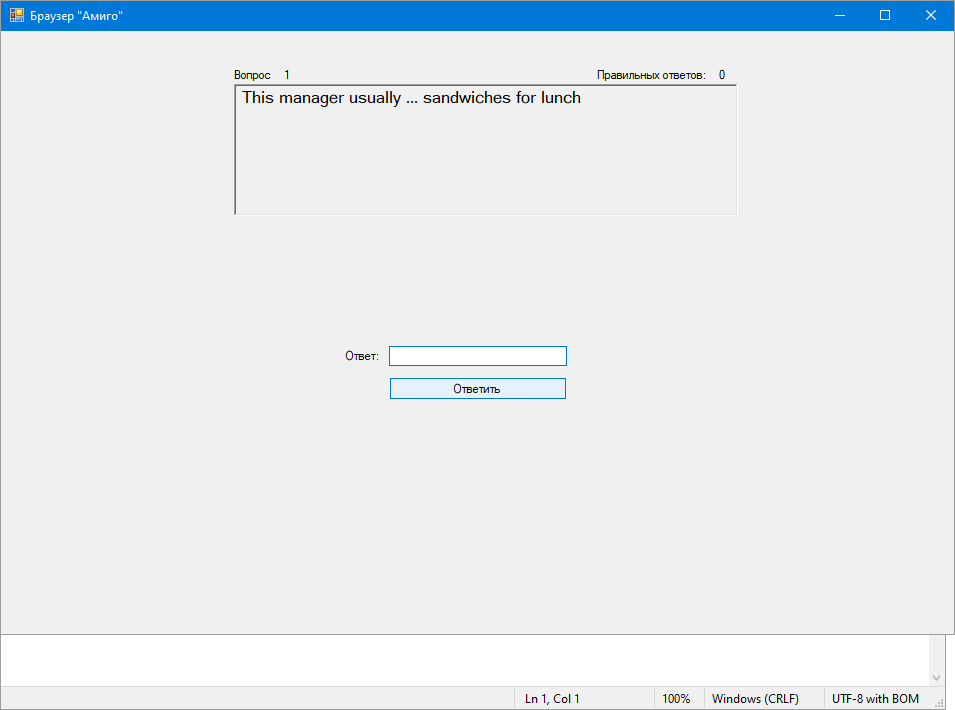
\includegraphics[scale=0.6]{task9/exec.png}
	\caption{Внешний вид окна после запуска приложения}
	\label{fig:exec9}
\end{figure}
Приложение содержит различные виды вопросов. Например, окно для вопросов с двумя вариантами
ответа выглядит следующим образом (см. рисунок \ref{fig:yesorno})
\begin{figure}[H]
    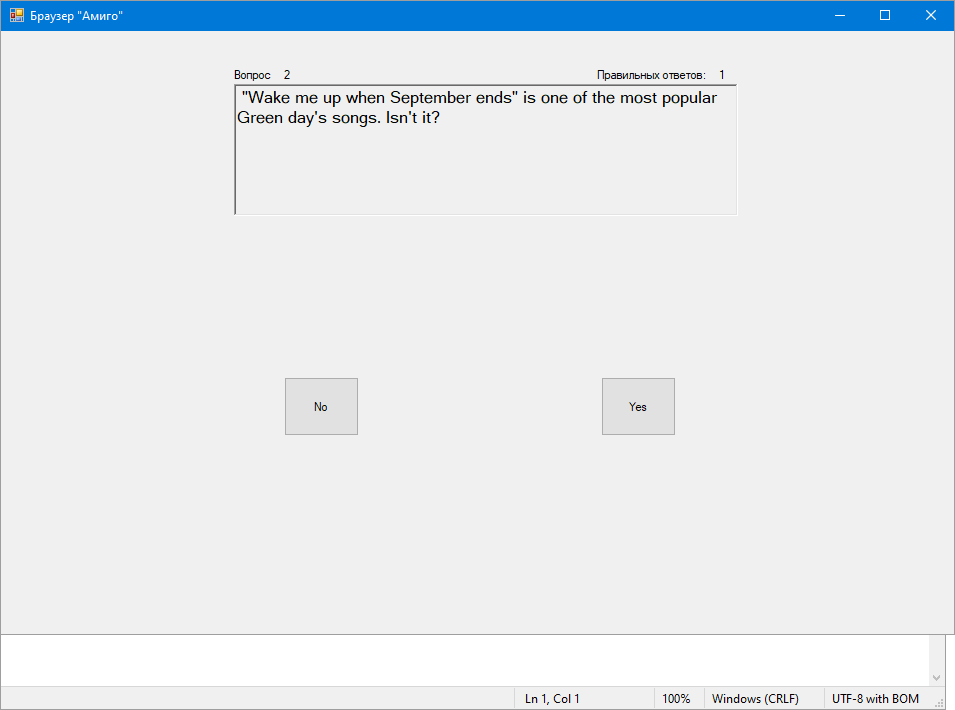
\includegraphics[scale=0.6]{task9/yesorno.png}
	\caption{Внешний вид для вопросов с двумя вариантами ответа}
	\label{fig:yesorno}
\end{figure}
В коде приложения была создана структура наследовования, которая
упрощает работу с различными вариантами вопросов:
\begin{minted}[fontsize=\small, breaklines=true, style=bw, linenos]{cpp}
ref struct Question {
	public: int questionId;
	public: Question() {};
	public: Question(int questionId, String^ text) : questionId(questionId), text(text) {};
	public: String^ text;
	public: virtual bool CheckAnswer() = 0;
	public: virtual Question^ Clone() = 0;
	};

ref struct ShortAnswerQuestion : Question {
	public: String^ expectedAnswer;
	public: String^ userAnswer;
	public: ShortAnswerQuestion() {};
	public: ShortAnswerQuestion(int questionId, String^ expectedAnswer) {
		this->questionId = questionId;
		this->expectedAnswer = expectedAnswer;
	}
	public: virtual bool CheckAnswer() override {
		return expectedAnswer->Equals(userAnswer);
	}
	public: virtual Question^ Clone() override {
		ShortAnswerQuestion^ obj = (gcnew ShortAnswerQuestion());
		obj->expectedAnswer = this->expectedAnswer;
		obj->questionId = this->questionId;
		obj->text = this->text;
		obj->userAnswer = this->userAnswer;
	Question^ toBeReturned = obj;
	return toBeReturned;
	}
};

ref struct SeveralAnswerQuestion : Question {
	public: int count;
	public: int userAnswerId;
	public: int expectedAnswerId;
	public: virtual bool CheckAnswer() override {
		return userAnswerId == expectedAnswerId;
	}
	public: SeveralAnswerQuestion() {};
	public: SeveralAnswerQuestion(int questionId, int expectedAnswer, int count) {
		this->questionId = questionId;
		this->expectedAnswerId = expectedAnswerId;
		this->count = count;
	}
	public: virtual Question^ Clone() override {
		SeveralAnswerQuestion^ obj = (gcnew SeveralAnswerQuestion());
		obj->expectedAnswerId = this->expectedAnswerId;
		obj->questionId = this->questionId;
		obj->text = this->text;
		obj->count = this->count;
		Question^ toBeReturned = obj;
		return toBeReturned;
	}
};
\end{minted}
В ходе выполнения программа сообщает пользователю о том, ввел 
ли он правильный ответ или нет (см. рисунки \ref{fig:whoops},\ref{fig:result9})
\begin{figure}[H]
    \centering
    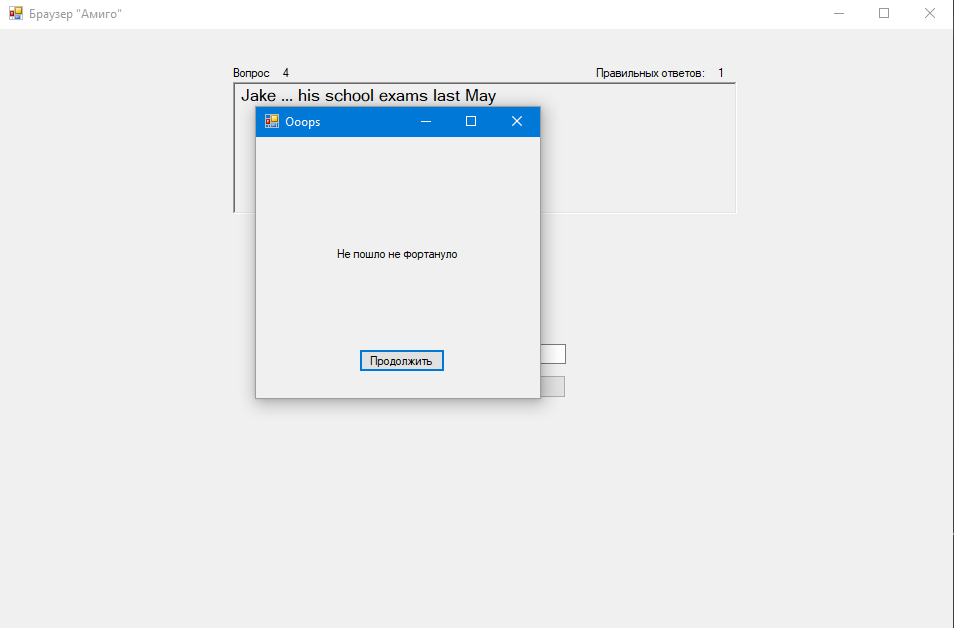
\includegraphics[scale=0.6]{task9/whoops.png}
	\caption{Окно в случае неправильного ответа на вопрос}
	\label{fig:whoops}
\end{figure}
\begin{figure}[H]
    \centering
    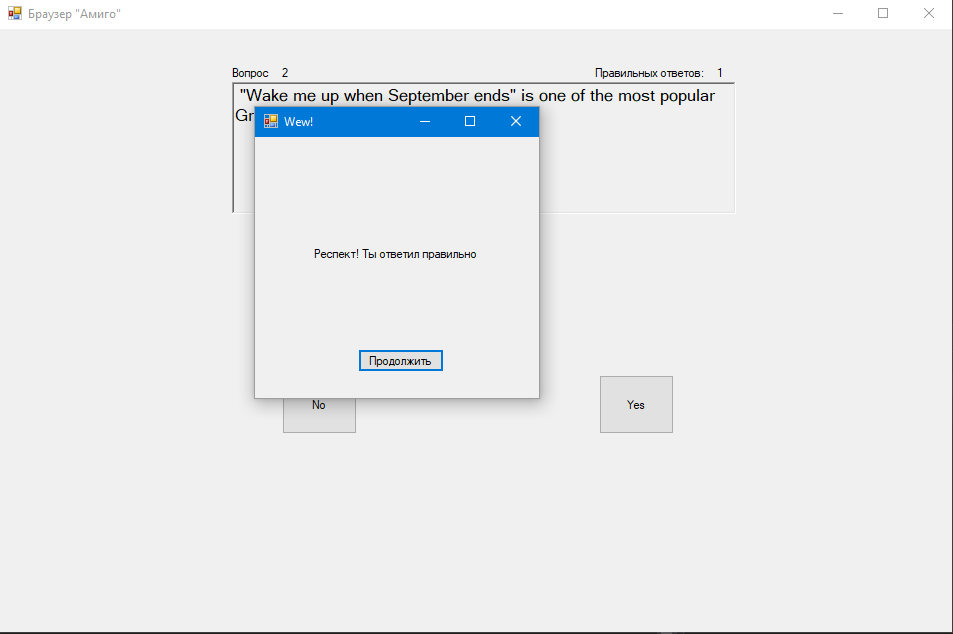
\includegraphics[scale=0.6]{task9/result.png}
	\caption{Окно в случае правильного ответа на вопрос}
	\label{fig:result9}
\end{figure}
Программа не содержит исключительных ситуаций, поэтому в их обработке нет необходимости.

Полный код программы приведен в приложении \ref{app:repos}.

